\documentclass{article}
\usepackage{listings}
\usepackage{amsmath}
\usepackage{fullpage}
\usepackage{tabularx}
\usepackage{graphicx}
\usepackage{tikz}
\usetikzlibrary{shapes.geometric, arrows}
\usepackage{cite}
\usepackage{hyperref}
\usepackage{float}
\begin{document}
\lstset{language=python, tabsize=4}
\title{Node mapping}
\author{Yuchen Hou \and Larry Holder}
\maketitle

\begin{abstract}
	We present node mapping, a technique created for link attribute prediction 
	tasks, powered by neural networks.
	This technique builds a neural net model, which learns to map every node in 
	a graph to a node vector of real numbers and learns to predict the target 
	link attribute using these node vectors.
	Every node vector contains information about the node related to the
	prediction task.
	The main idea is to convert nodes (categorical variables) to vectors 
	(numerical variables), as neural nets can directly handle only numerical 
	variables.
\end{abstract}

\section{Introduction}

\subsection{Background}
We have seen the wide spread success of neural networks since 2010, as they are 
becoming state-of-the-art models in a growing number of application domains of 
machine learning, (e.g., speech recognition \cite{hannun2014deep}, image 
recognition \cite{simonyan2014very}, and natural language 
processing \cite{yao2013recurrent}).
These neural net models not only achieved higher prediction accuracy than 
traditional models, but also require much less domain knowledge and engineering.
In 2016, Google AlphaGo AI - powered by neural net and Monte Carlo tree search 
- defeated go champion Lee Sedol, demonstrated how a statistical approach can 
complement logical approaches in solving challenging 
problems \cite{silver2016mastering}.
Specifically, in a game like go with simple rules but too many possible 
configurations to explore, neural net models achieve good results with 
reasonable computing resources, which are easily exhausted by algorithms solely 
powered by search.

\subsection{Motivation}
As neural nets have demonstrated their power in many domains, we naturally 
wonder if we can apply them in prediction tasks in graph mining domain, and 
what kind of techniques are helpful in using their power.
There are existing techniques with promising results already.
Two earlier attempts were graph neural nets and relational neural 
nets \cite{scarselli2009graph}, where neural nets are incorporated into a 
traditional iterative graph information propagation approach.
A later attempt was deep walk \cite{perozzi2014deepwalk}, where a graph is 
reduced to a natural language corpus so that existing neural net models 
designed for natural language processing can handle the graph.
We find these techniques complex, indirect and unable to fully use rich graph 
information in real applications, e.g. making recommendations for social 
network users based on user activities like messaging friends, commenting 
articles, and rating movies.
However, these attempts all include an essential step of applying neural net in 
graphs: converting graph to numerical variables.
This step is essential in other application domains as well, because neural 
nets cannot directly handle non-numerical variables.

\subsection{Goal}
We want to create a technique to predict link attributes in a graph using a 
neural net model. The graph can have any topology and its links can have any 
number of numerical(including boolean) attributes. The technique should build a 
neural net model, which learns to represent the graph in a meaningful way and 
to predict the target link attribute using the representation it learns.

\section{Observations and approach}

\subsection{Entities, representations and relations in different domains}
In order to understand how a neural net can handle prediction tasks in graphs, 
we take an overview on 3 types entities in these 3 domains and in graph mining. 
\autoref{tab:domains} provides a summary of these entities, their 
representations in neural nets and inter-entity relation examples in these 
domains.
\begin{table}[h]
	\centering
	\begin{tabularx}{\textwidth}{ |c|c|c|X| }
		\hline domain & entity & representation & relations to other entities 
		\\ 
		\hline image recognition & image & 2D light intensity array & NA \\ 
		\hline speech recognition & utterance/spectrogram & 2D sound intensity 
		array & NA \\ 
		\hline natural language & word & word vector & relations to other words 
		\\ 
		\hline graph & movie & node vector & directed by director, etc \\ 
		\hline graph & user & node vector & rate movies, etc \\
		\hline
	\end{tabularx}
	\caption{A summary of various types of entities, their numerical 
	representations and inter-entity relations in different domains: images and 
	utterances can be directly represented by 2D numerical arrays, but have no 
	strong relations to other images or utterances; words and various types of 
	nodes in graphs can represented by 1D numerical arrays(which will be 
	introduced below), and have strong relations to other words and nodes. 
	Notice that the representations for all the entities are numerical arrays, 
	because neural nets rely on neurons' activations and communications, which 
	are both numerical.}
	\label{tab:domains}
\end{table}
The entities listed in the lower rows have increasing 
representation complexities.
Images and utterances(spectrograms) can be naturally represent as 2D numerical 
arrays, which makes them easy for neural net to process.
Words are categorical variables and consequently harder, but 
they can be mapped to 1D numerical arrays (i.e. word vectors) by word2vec 
technique so neural nets can still process them \cite{mikolov2013efficient}.

\subsection{Learning word vectors}
Interestingly, it turns out neural net itself has the capability to do the 
mapping.
In word2vec, a neural net learns to map every word to a vector without any 
domain knowledge.
\autoref{tab:word} shows how each word in a vocabulary is represented by a word 
vector.
\begin{table}[h]
	\centering
	\begin{tabularx}{0.5\textwidth}{|X|X|} \hline
		word ID & word vector \\ \hline
		1 & [2.3, 564, -9.5 ... 3] \\ \hline
		2 & [76, -342.2, 0.3 ... 4.2] \\ \hline
		3 & [-345, -834, 0.3 ... 34] \\ \hline
		... & ... \\ \hline
		n & $ [x_1, x_2, x_3 ... x_d] $ \\ \hline
	\end{tabularx}
	\caption{Word vector table in a vocabulary of size n and word vectors with 
	size d: 
	Each word has an ID and its spelling is now shown;
	each vector is randomly initialized before learning and then gradually 
	updated by the neural net during learning.}
	\label{tab:word}
\end{table}
In a corpus, every word is described/defined only by related 
words in its context, although relations between the words are implicit. 
Nonetheless, the neural net can learn from word co-occurrences and map words 
accordingly such that the relations between words are preserved in the vector 
space \cite{mikolov2013distributed}.

\subsection{Learning node vectors}

If we compare language data and graph data, we can immediately realize they 
have many similarities, shown in \autoref{tab:wordVSnode}.
\begin{table}[h]
	\centering
	\begin{tabularx}{\textwidth}{ |X|X|X| } \hline
		aspect  & natural language processing & graph mining \\ \hline
		dataset & corpus & graph \\ \hline
		basic entities & words & nodes \\ \hline
		entity collection & vocabulary & node set \\ \hline
		relations & co-occurrences (implicit) & links (explicit) \\ \hline
		representation & word vectors & node vectors \\ \hline
	\end{tabularx}
	\caption{A comparison of language data and graph data from 
		several aspects: these similarities suggest a neural net might be able 
		to map nodes to node vectors just like mapping words to word vectors.}
	\label{tab:wordVSnode}
\end{table}
Word and node vectors are similar to feature vectors. We didn't use the term 
feature vector to avoid any implication of feature engineering with domain 
knowledge. Typically, the attributes of words and nodes are not observable so 
neural nets need to learn these vectors from the relations between words and 
nodes.
Apparently, mapping node to node vectors should be more direct than mapping 
word to word vectors, because the relations between nodes are explicit(i.e., 
link and link attributes), while relations between words are implicit(i.e., 
word co-occurrences). In a social network example, the rating a movie received 
from a user explicitly tells us how much the user likes that movie; the number 
of messages a user sends to another user explicitly tells us how close they are 
connected. In a corpus example, the co-occurrences of words [the, quick, brown, 
fox, jumps, over] implicitly suggest these words may be related but do not tell 
us what their relations are. This means the neural net should be able to learn 
node mapping supervised by the link attributes in a more direct way than it 
learns word mapping supervised by word co-occurrences.

\section{Application scenario}

\subsection{Recommendations in a social network}
We demonstrate a usage example of node mapping in social network: making 
recommendations to users.
This is a simplified social network where users can send messages to other 
users and give ratings to movies.
The service provider is interested in recommending friends and movies for each 
user, solely based on how much he communicates to other users and how much 
he likes different movies.
Formally, the graph is:
\begin{itemize}
	\item a node set consisting of 2 types of nodes: users and movies
	\item a link set consisting of 2 types of links: user-user links with 
	numerical attribute called messages indicating the amount of messages the 
	user has sent to the other 	user(e.g., total number of messages, words 
	or characters),
	and user-movie links with numerical attribute called rating indicating the 
	rating the user has given to the movie(e.g., a number in range(0, 5))
\end{itemize}
If we can build a model to predict the messages attribute of user-user links(or 
the rating attribute of user-movie links), we can know how much a user would 
like each of the users(movies) he has not connected to (rated) and recommend 
those he would like the most.
Formally, the prediction task is:
\begin{itemize}
	\item input: X = (node1, node2)
	\item output: Y = link(node1, node2).attribute
\end{itemize}
Node mapping technique is created to perform this task. In the following, we 
will demonstrate how to use this technique in rating prediction. We also expect 
it (with moderate modifications) to work for messages prediction, but we 
currently haven't verified that experimentally.

\subsection{Dataset: MovieLens 100K}
We use MovieLens 100k dataset \cite{harper2015movielens} 
\footnote{http://grouplens.org/datasets/movielens/100k/} to verify the 
functionality of node mapping. This dataset has the following specs
\begin{itemize}
	\item number of users: 1000
	\item number of movies: 1700
	\item number of ratings: 100,000
\end{itemize}
and a few samples are shown in \autoref{tab:rating}.
\begin{table}[h]
	\centering
	\begin{tabularx}{0.5\textwidth}{ |X|X|X| }  \hline
		user ID & movie ID & rating \\ \hline
		0 & 355 & 4 \\ \hline
		0 & 876 & 3 \\ \hline
		0 & 232 & 5 \\ \hline
		1 & 324 & 2 \\ \hline
		... & ... & ... \\ \hline
	\end{tabularx}
	\caption{The Movie Lens dataset: Every link has 1 numerical attribute - 
	rating.}
	\label{tab:rating}
\end{table}
The dataset is split into 3 sets as in normal machine learning experiments:
\begin{itemize}
	\item training set: 70\%
	\item validation set: 10\%
	\item test set: 20\%
\end{itemize}

\subsection{Prediction task: rating prediction}
The model will need to predict the ratings in the testing set: given any (user, 
movie) pair, it needs to predict the rating given to the movie by the user:
\begin{itemize}
	\item input: X = (user, movie)
	\item output: Y = rating(user, movie)
\end{itemize}

\section{Implementation}
Node mapping technique builds a fully-connected neural net model, shown 
in \autoref{fig:nodeMapping}.
\begin{figure}[H]
	\centering
	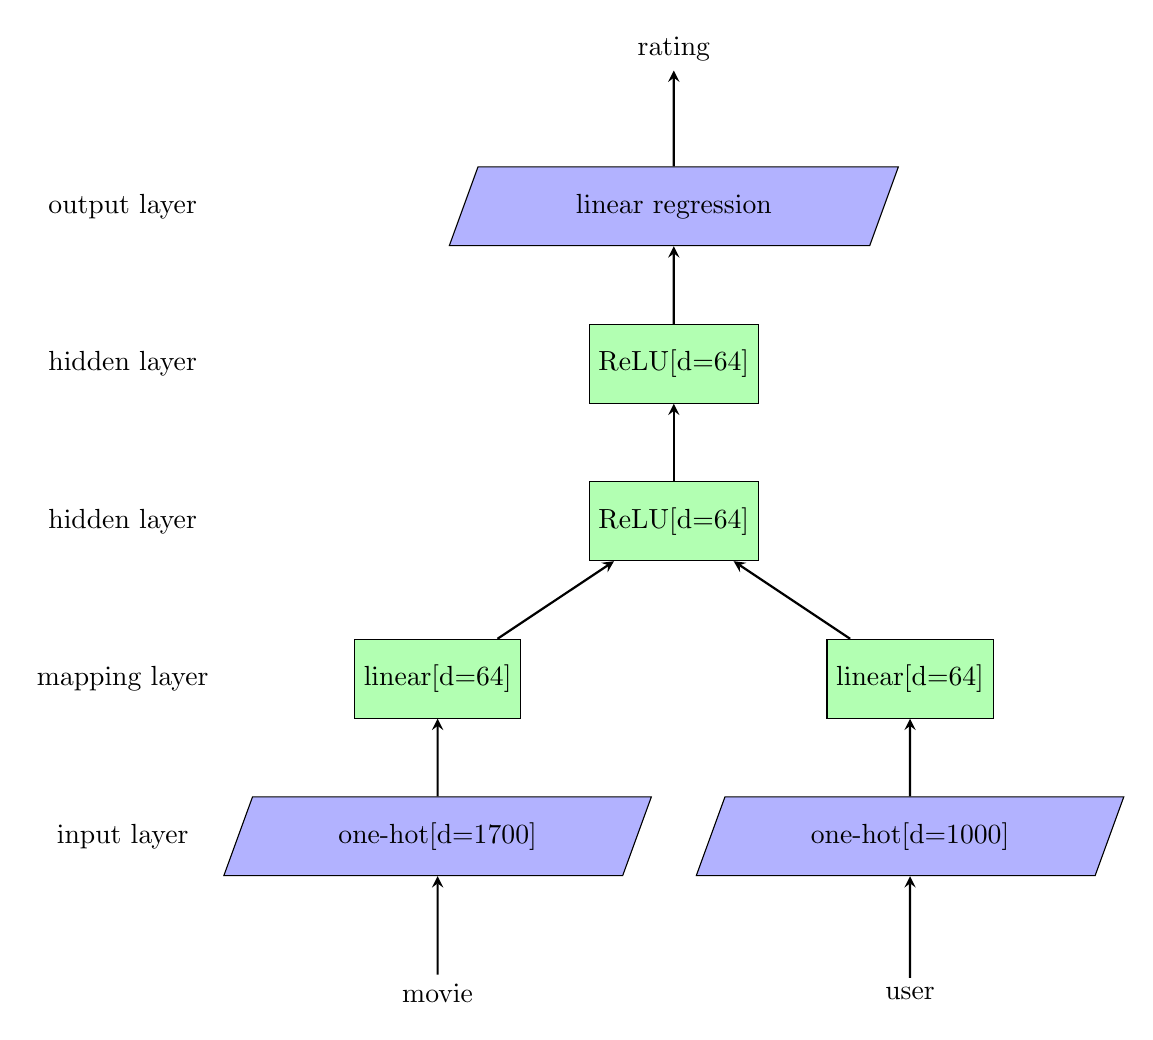
\begin{tikzpicture}[node distance=2cm]
	\tikzstyle{io} = [trapezium, trapezium left angle=70, trapezium right 
	angle=110, minimum width=1cm, minimum height=1cm, text centered, 
	draw=black, fill=blue!30]
	\tikzstyle{process} = [rectangle, minimum width=1cm, minimum height=1cm, 
	text centered, draw=black, fill=green!30]
	\tikzstyle{arrow} = [thick,->,>=stealth]
	\node (linearRegression) [io] {linear regression};
	\node (relu2) [process, below of=linearRegression] {ReLU[d=64]};
	\node (relu3) [process, below of=relu2] {ReLU[d=64]};
	\node (linear2) [process, below of=relu3, xshift=-3cm] {linear[d=64]};
	\node (linear1) [process, below of=relu3, xshift=3cm] {linear[d=64]};
	\node (oneHot2) [io, below of=linear1] {one-hot[d=1000]};
	\node (oneHot1) [io, below of=linear2] {one-hot[d=1700]};
	\node (rating) [above of=linearRegression] {rating};
	\node (output) [left of=linearRegression, xshift=-5cm] {output layer};
	\node (hidden2) [below of=output] {hidden layer};
	\node (hidden1) [below of=hidden2] {hidden layer};
	\node (mapping) [below of=hidden1] {mapping layer};
	\node (input) [below of=mapping] {input layer};
	\node (movie) [below of=oneHot1] {movie};
	\node (user) [below of=oneHot2] {user};
	\draw [arrow] (movie) -- (oneHot1);
	\draw [arrow] (user) -- (oneHot2);
	\draw [arrow] (oneHot2) -- (linear1);
	\draw [arrow] (oneHot1) -- (linear2);
	\draw [arrow] (linear1) -- (relu3);
	\draw [arrow] (linear2) -- (relu3);
	\draw [arrow] (relu3) -- (relu2);
	\draw [arrow] (relu2) -- (linearRegression);
	\draw [arrow] (linearRegression) -- (rating);
	\end{tikzpicture}	
	\caption{The 5-layer fully-connected neural net model for a dataset with 
	1700 movies and 1000 users with layer size 64: The d in the bracket 
	refers to dimension, the layer's size (number of units in the layer).
	We keep all layers the same size for simplicity, although layers of 
	different sizes may produce better results.
	The text before the bracket refers to the activation function of the units 
	in the layer(except for one-hot, which refers to the activations 
	themselves).
	Only layers and their connections are shown, while the units in each layer 
	and their connections are not shown.}
	\label{fig:nodeMapping}
\end{figure}
The model contains following layers:
\begin{itemize}
	\item an input layer with one-hot activations: it has 1 channel for movies 
	and 1 channel for users;
	the activations of units in this layer are driven by brute force(e.g., for 
	the 42nd movie, the movie input layer will have 1 at the 42nd unit and 0 at 
	other units)
	\item a mapping layer with linear units: it has 2 channels to map each 
	movie (and each user) node to a vector(hence the name node mapping);
	the activations of units of these 2 channels form the 2 node vectors(i.e., 
	movie vector and user vector);
	it is the most critical layer as it gradually learns to map every node to 
	the correct vector during training(learning information about users and 
	movies from ratings);
	\item several hidden layers(2 layers are shown in the figure) of 
	ReLU(rectified linear unites):
	they have non-linear activation functions to give the model sufficient 
	complexity; 
	they learn to process node vectors and produce more abstract and 
	rating-relevant information (learning how different factors of each user 
	and movie are related);
	\item an output layer with a linear regression unit: learn to predict the 
	rating based on processed information;
\end{itemize}
We have an open source implementation available for interested readers and we 
are open to collaborations \footnote{https://github.com/yuchenhou/elephant}.
We build an estimator with the above neural net model and popular training 
techniques for neural net including SGD(stochastic gradient descent) and its 
variant Adagrad(advanced gradient descent), mini-batch, and dropout.
The code is in Python and TensorFlow \cite{tensorflow2015-whitepaper} 
is the main machine learning package.
One thing to notice is that the actual implementation of the input layer is a 
little more complex than the conceptual one-hot logic: it handles nodes like 
words.
Word is treated as a categorical variable with n discrete 
values(categories) in a vocabulary of size n, as shown in \autoref{tab:word}.
Every time we feed a word(a node) to the estimator, we actually feed the word 
ID to it. The estimator uses the ID to index the word vector table, retrieve 
the word vector and directly activate the mapping layer using this vector. 
During learning, these vectors are updated the same way weights are updated.
In other words, in the actual implementation, the 2 channels in the input layer 
are movie and user tables: the inputs are the movie and user IDs; the outputs 
are movie and user vectors, directly fed to the mapping layer.

\section{Experiments}

\subsection{Process}
The estimator learns for several epochs.
During each epoch, the it updates its model by fitting the training set, and 
then evaluates the progress by performing prediction using the validation set.
It logs the average training error and validation error for each epoch and 
stops learning when the validation error starts increasing to reduce 
over-fitting.
After learning, it evaluates the its model by performing prediction using the 
testing set.
We use MAE(mean absolute error) as the metric for training, validation and 
testing errors.
\autoref{fig:trainnig} shows an example learning process.
\begin{figure}[H]
	\centering
	\includegraphics[width=0.5\linewidth]{training}
	\caption{An example learning process of 11 epochs(starting from epoch 0): 
	The estimator stopped learning at epoch 10 when validation error started 
	increasing.}
	\label{fig:trainnig}
\end{figure}

\subsection{Prediction accuracy}
The estimator's prediction error for the specific dataset observed in the 
experiments is in range [0.69, 0.72], depending on the hyper parameters of the 
estimator.
This is consistently lower than the state-of-the-art prediction error 0.740 
achieved by collaborative filtering and category experts methods on this 
dataset \cite{hwang2016efficient}.
Also, the estimator is very robust against hyper parameter changes, as shown in 
\autoref{tab:robust}.
\begin{table}[h]
	\centering
	\begin{tabularx}{\textwidth}{ |c|c|c|c|c|X| } \hline
		optimizer  & learning rate & dropout(keep probability) & layer size & 
		number of layers & 
		testing error \\ \hline
		SGD & 0.01 & 0.9 & 64 & 2 & 0.7009 \\ \hline
		SGD & 0.01 & 0.9 & 64 & 1 & 0.7129 \\ \hline
		SGD & 0.01 & 0.9 & 64 & 4 & 0.7151 \\ \hline
		SGD & 0.01 & 0.9 & 32 & 2 & 0.7120 \\ \hline
		SGD & 0.01 & 0.9 & 128 & 2 & 0.7177 \\ \hline
		SGD & 0.01 & 0.8 & 64 & 2 & 0.7007 \\ \hline
		SGD & 0.01 & 0.6 & 64 & 2 & 0.6956 \\ \hline
		SGD & 0.1 & 0.6 & 64 & 2 & 0.7019 \\ \hline
		SGD & 0.05 & 0.6 & 64 & 2 & 0.6985 \\ \hline
		Adagrad & 0.05 & 0.6 & 64 & 2 & 0.7143 \\ \hline
		Adagrad & 0.01 & 0.6 & 64 & 2 & 0.7109 \\ \hline
		Adagrad & 0.1 & 0.6 & 64 & 2 & 0.7114 \\ \hline
		Adagrad & 0.1 & 0.8 & 64 & 2 & 0.7058 \\ \hline
		Adagrad & 0.1 & 0.9 & 64 & 2 & 0.6925 \\ \hline
		Adagrad & 0.1 & 0.9 & 32 & 2 & 0.6965 \\ \hline
		Adagrad & 0.1 & 0.9 & 128 & 2 & 0.7026 \\ \hline
		Adagrad & 0.1 & 0.9 & 32 & 1 & 0.7032 \\ \hline
		Adagrad & 0.1 & 0.9 & 32 & 4 & 0.7008 \\ \hline
	\end{tabularx}
	\caption{High robustness of the estimator against hyper parameter changes: 
	the estimator maintains very low testing error for a wide range of 
	parameter configurations.}
	\label{tab:robust}
\end{table}

\section{Strengths of this approach}
This technique has the following strengths:
\begin{enumerate}
	\item low complexity: it is simple and scalable
	\item high flexibility: it can learn from and predict rich node and link 
	attributes
	\item high efficiency: it is very streamlined online learning without any 
	expensive graph operations(not even neighbor node lookup or random walk)
\end{enumerate}
\subsection{Representing nodes as node vectors}
This technique is a node-centric approach in terms of information flow, as 
information about nodes is extracted from links connecting these nodes and then 
stored in nodes.
This fits many real world graphs well: usually a graph has complex entities 
with unobservable attributes which we represent as nodes; it also has simple 
interactions/relations between these entities with observable attributes which 
we represent as links, as shown in \autoref{tab:nodesVSlinks}.
In the above application scenario, this means who a user contacts and what 
movies a user likes tells us what kind of person this user is.
\begin{table}[h]
	\centering
	\begin{tabularx}{0.5\textwidth}{ |c|X|X| } \hline
		aspect  & node & link \\ \hline
		complexity & high & low \\ \hline
		observability & low & high \\ \hline
		example & user & activities \\ \hline
	\end{tabularx}
	\caption{A comparison of nodes and links with respect to their complexity 
		and attribute observability:
		links tend to have low complexity and high attribute observability 
		while nodes are the opposite.
		In a social network example,
		it's easy to observe simple user activities like sending messages other 
		users,
		leaving comments on posts and give ratings to music,
		but it's hard to observe complex user attributes like personality, 
		style or taste in movies.}
	\label{tab:nodesVSlinks}
\end{table}

\subsection{Online learning}
This technique never requires the construction or storage of the graph and fits 
streaming graph scenarios.
The training samples in this approach are links in the graph.
During each training step, the neural net extracts the information in the link 
and uses it to update the node vector.
After each training step, the sample can be discarded.
Therefore, the learning is incremental and only requires samples of different 
walks in the graph, not the construction or storage of the complete graph.
In practice, it is sufficient to cache a finite number of latest links streamed 
in inside the memory for learning using SGD with mini-batch.

\section{Future work}
\begin{enumerate}
	\item unable to handle non-numerical attributes: e.g., a message from user 
	A to user B (a link from A to B) or an article (a node) contain texts 
	(string attributes), which this technique cannot directly handle
\end{enumerate}

\section{Conclusions}
Node mapping is a efficient technique for link attribute prediction using 
neural net models.
It can achieve state-of-the-art prediction accuracy using reasonable amount of 
computing resources.
For recommendation tasks in social networks, this technique provides a 
promising neural net approach:
understand complex users from their simple activities, map users to 
vectors and use the vectors to predict their activities.

\bibliographystyle{acm}
\bibliography{references}

\end{document}
